\section{Sample normalized variation as a measure of roughness}
    \subsection{Theoretical parameters}
        Let us consider a sequence of partitions $\pi^n$ of $\left[0, T\right]$ with 
        $\left|\pi^n\right|:=\max_{t_i^n \in \pi^n} (t_{i+1}^n - t_i^n) \to 0$. 
        \begin{definition}
            A function $x \in C[0, T]$ is said to have the finite $p$-th variation along the sequence of partitions $\pi^n$ 
            if there exists a continious increasing function $\left[x\right]_{\pi}^{(p)}$ such that for all subpartitions $\tilde\pi^n(t) = \pi^n \cap [0, t]$
            \begin{equation}
                \sum_{t_i^n \in \tilde\pi^n(t)} \left|x(t_{i+1}^n) - x(t_i^n)\right|^p \to \left[x\right]_{\pi}^{(p)}(t), \quad n\to \infty,
            \end{equation}
            and the set of all functions having finite $p$-th variation along $\pi$ we denote $V_\pi^p$.
        \end{definition}
        \begin{definition}
            The \emph{variation index} of a path $x$ is defined as $p^\pi(x) := \inf \left\{p\geq 1 \colon \quad x\in V_\pi^p\right\}$, and the \emph{roughness index} is defined as $H^\pi(x):=\frac{1}{p^\pi(x)}$.
        \end{definition}
        It has been proven that for fBm with Hurst parameter $H$ $p^\pi(W^H) = \frac{1}{H}$ and $H^\pi(W^H) = H$.
        
        \begin{definition}
            $x\in V_\pi^p$ is said to have $p$-th normalized variation if there exists such continious function $w(x, p, \pi)\colon [0, T] \to \mathbb{R}$ that
            \begin{equation}
                \sum_{\tilde\pi^n(t)}\frac{\left|x(t_{i+1}^n) - x(t_i^n)\right|^p}{\left[x\right]_{\pi}^{(p)}(t_{i+1}^n)-\left[x\right]_{\pi}^{(p)}(t_i^n)} (t_{i+1}^n-t_{i}^n) \to w(x, p, \pi).
            \end{equation}
        \end{definition}

        From Theorem 2.4 \cite{Cont2022}, it is known that the variation index must be found as a solution of 
        \begin{equation}
            w(x, p, \pi) = t.
        \end{equation}
    \subsection{The $W$ Statistic}
        \begin{figure}[htbp]
            \centering
            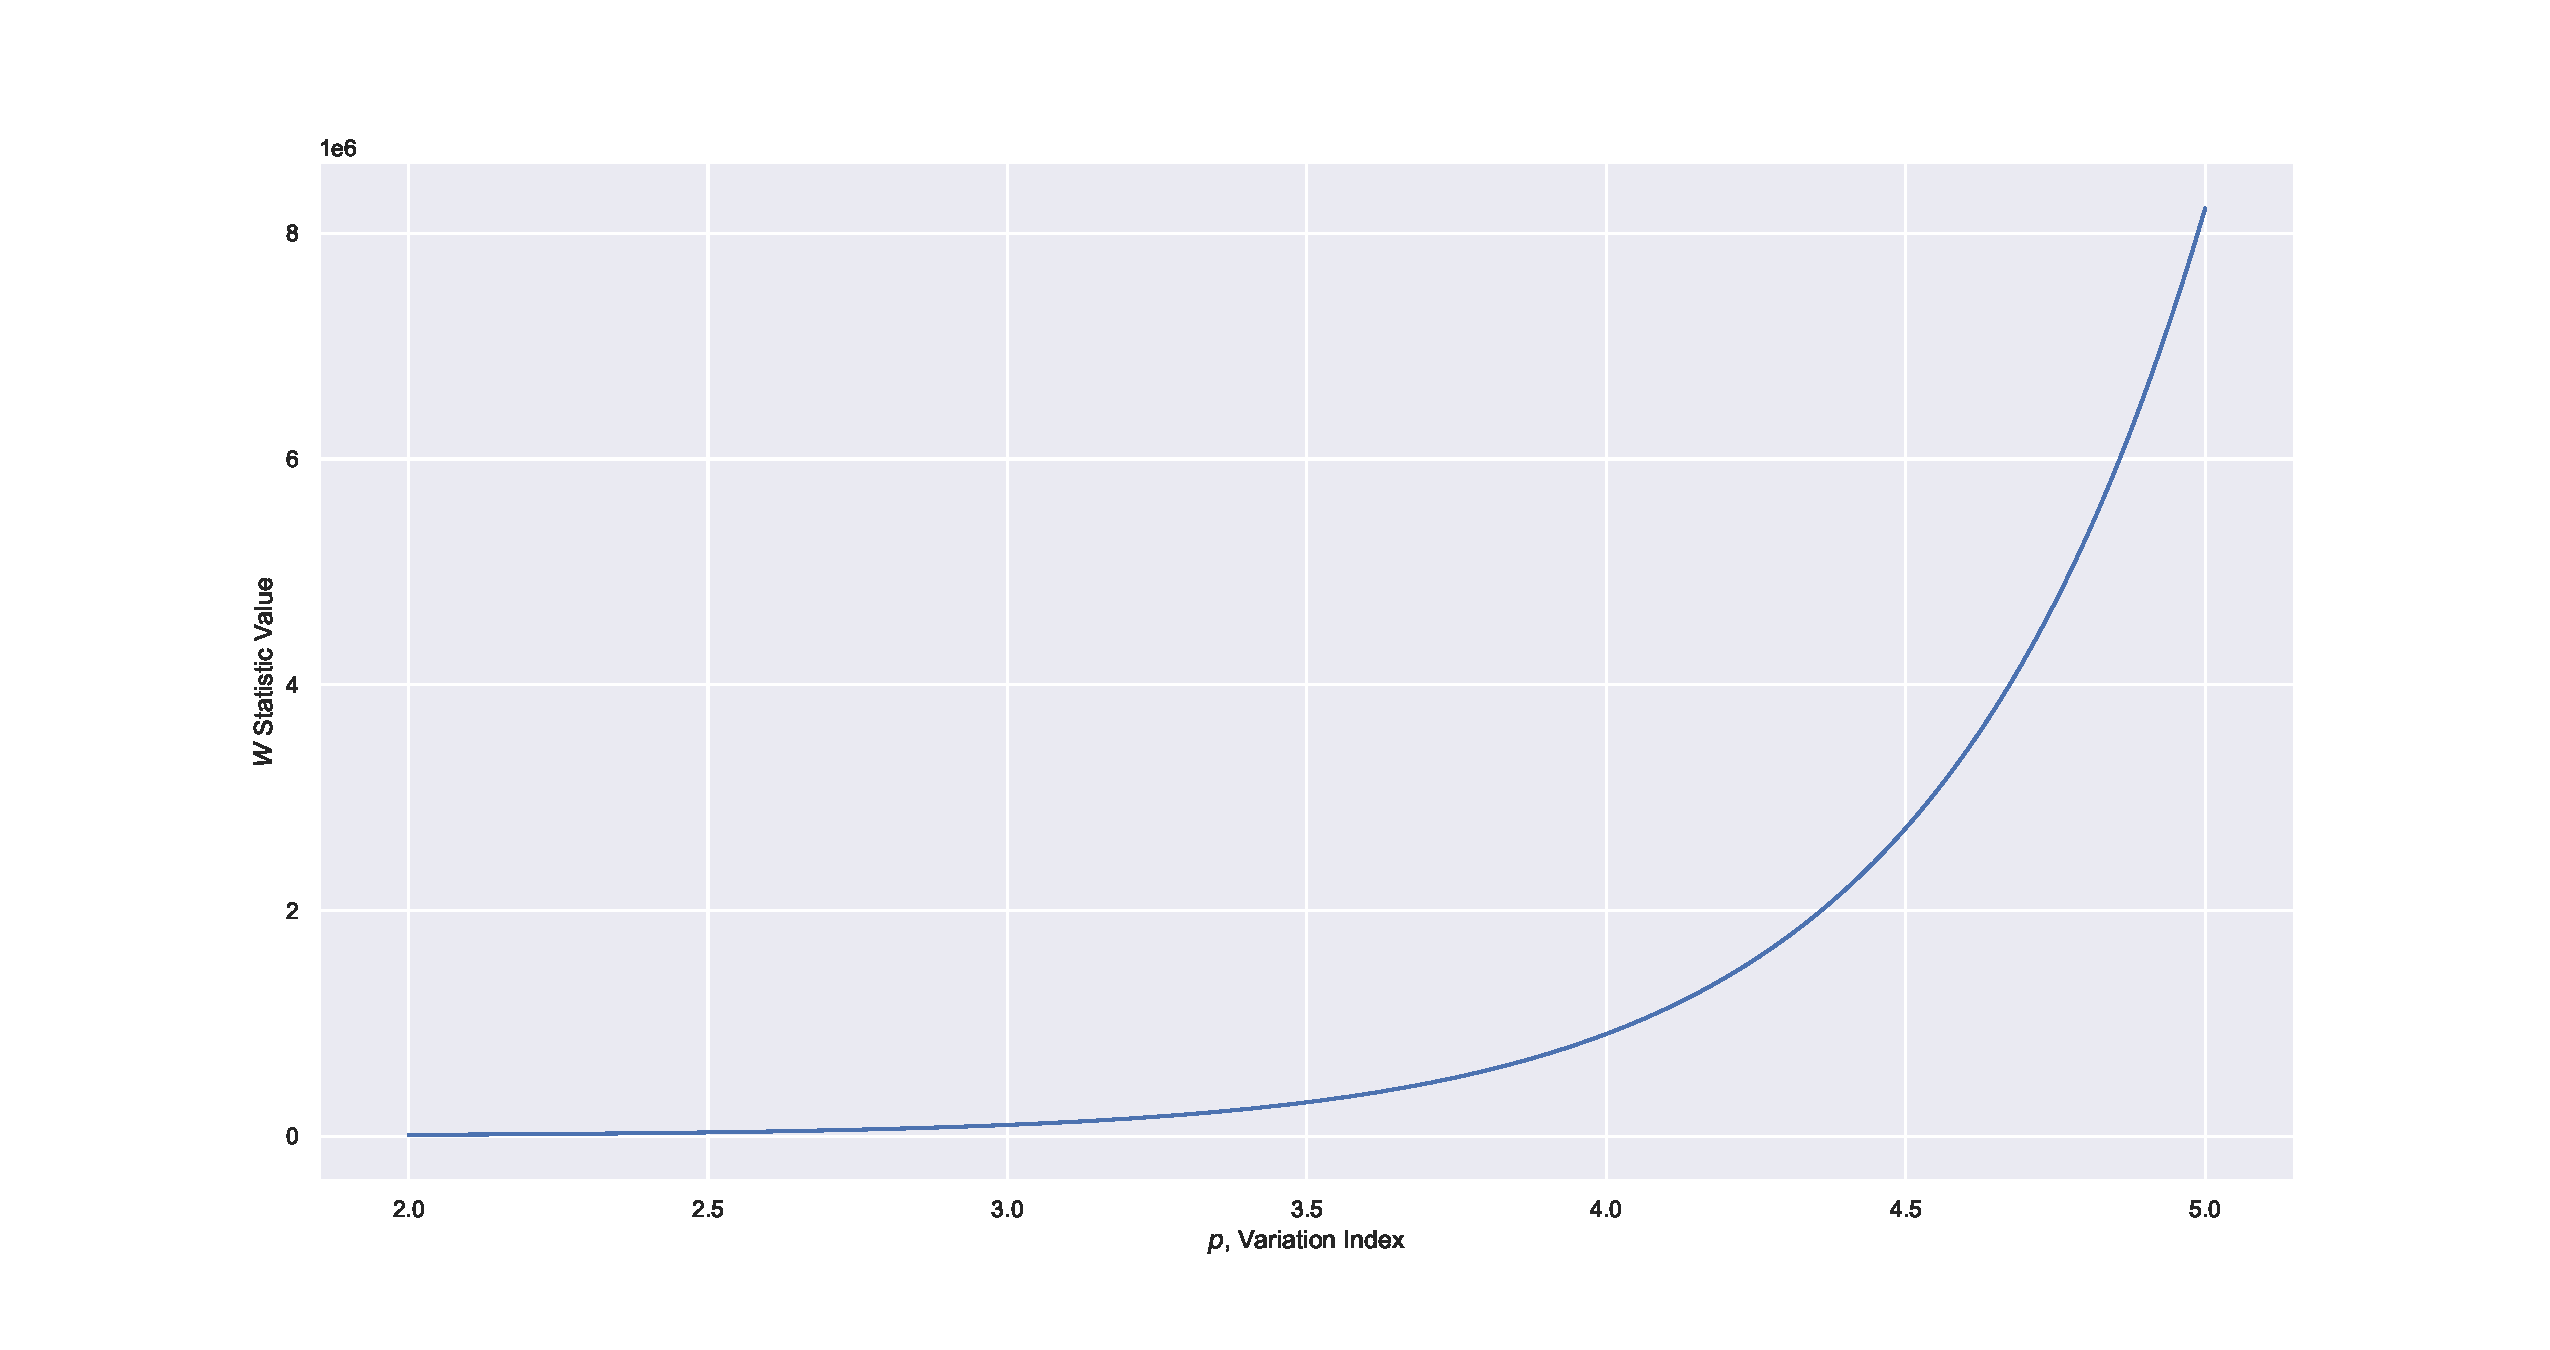
\includegraphics[width=\linewidth]{fig/W Stat Illustration.pdf}
            \caption{The $W$ statistic illustration as a function of $p$}
        \end{figure}

        Let us consider $\pi^L$, $\pi^K$ -- partitions with sampling frequencies $L\gg K$ ($\pi^K \subset \pi^L$).
        \begin{definition}
            Sample normalized $p$-th variation is defined as
            \begin{equation}
                W(L, K, p, t, X) = \sum_{\tilde\pi^K(t)}\frac{\left|x(t_{i+1}^K) - x(t_i^K)\right|^p}{\sum_{t_i^n \in \tilde\pi^n(t)} \left|x(t_{i+1}^n) - x(t_i^n)\right|^p} (t_{i+1}^n-t_{i}^n)
            \end{equation}
        \end{definition}

\section{Roughness estimation of Monte-Carlo simulations}

    \subsection{Brownian and fractional Brownian motion}
        We shall test our method on those processes, whose roughness is well-known.
        \subsubsection{Brownian motion}
            \begin{figure}[htbp]
                \centering
                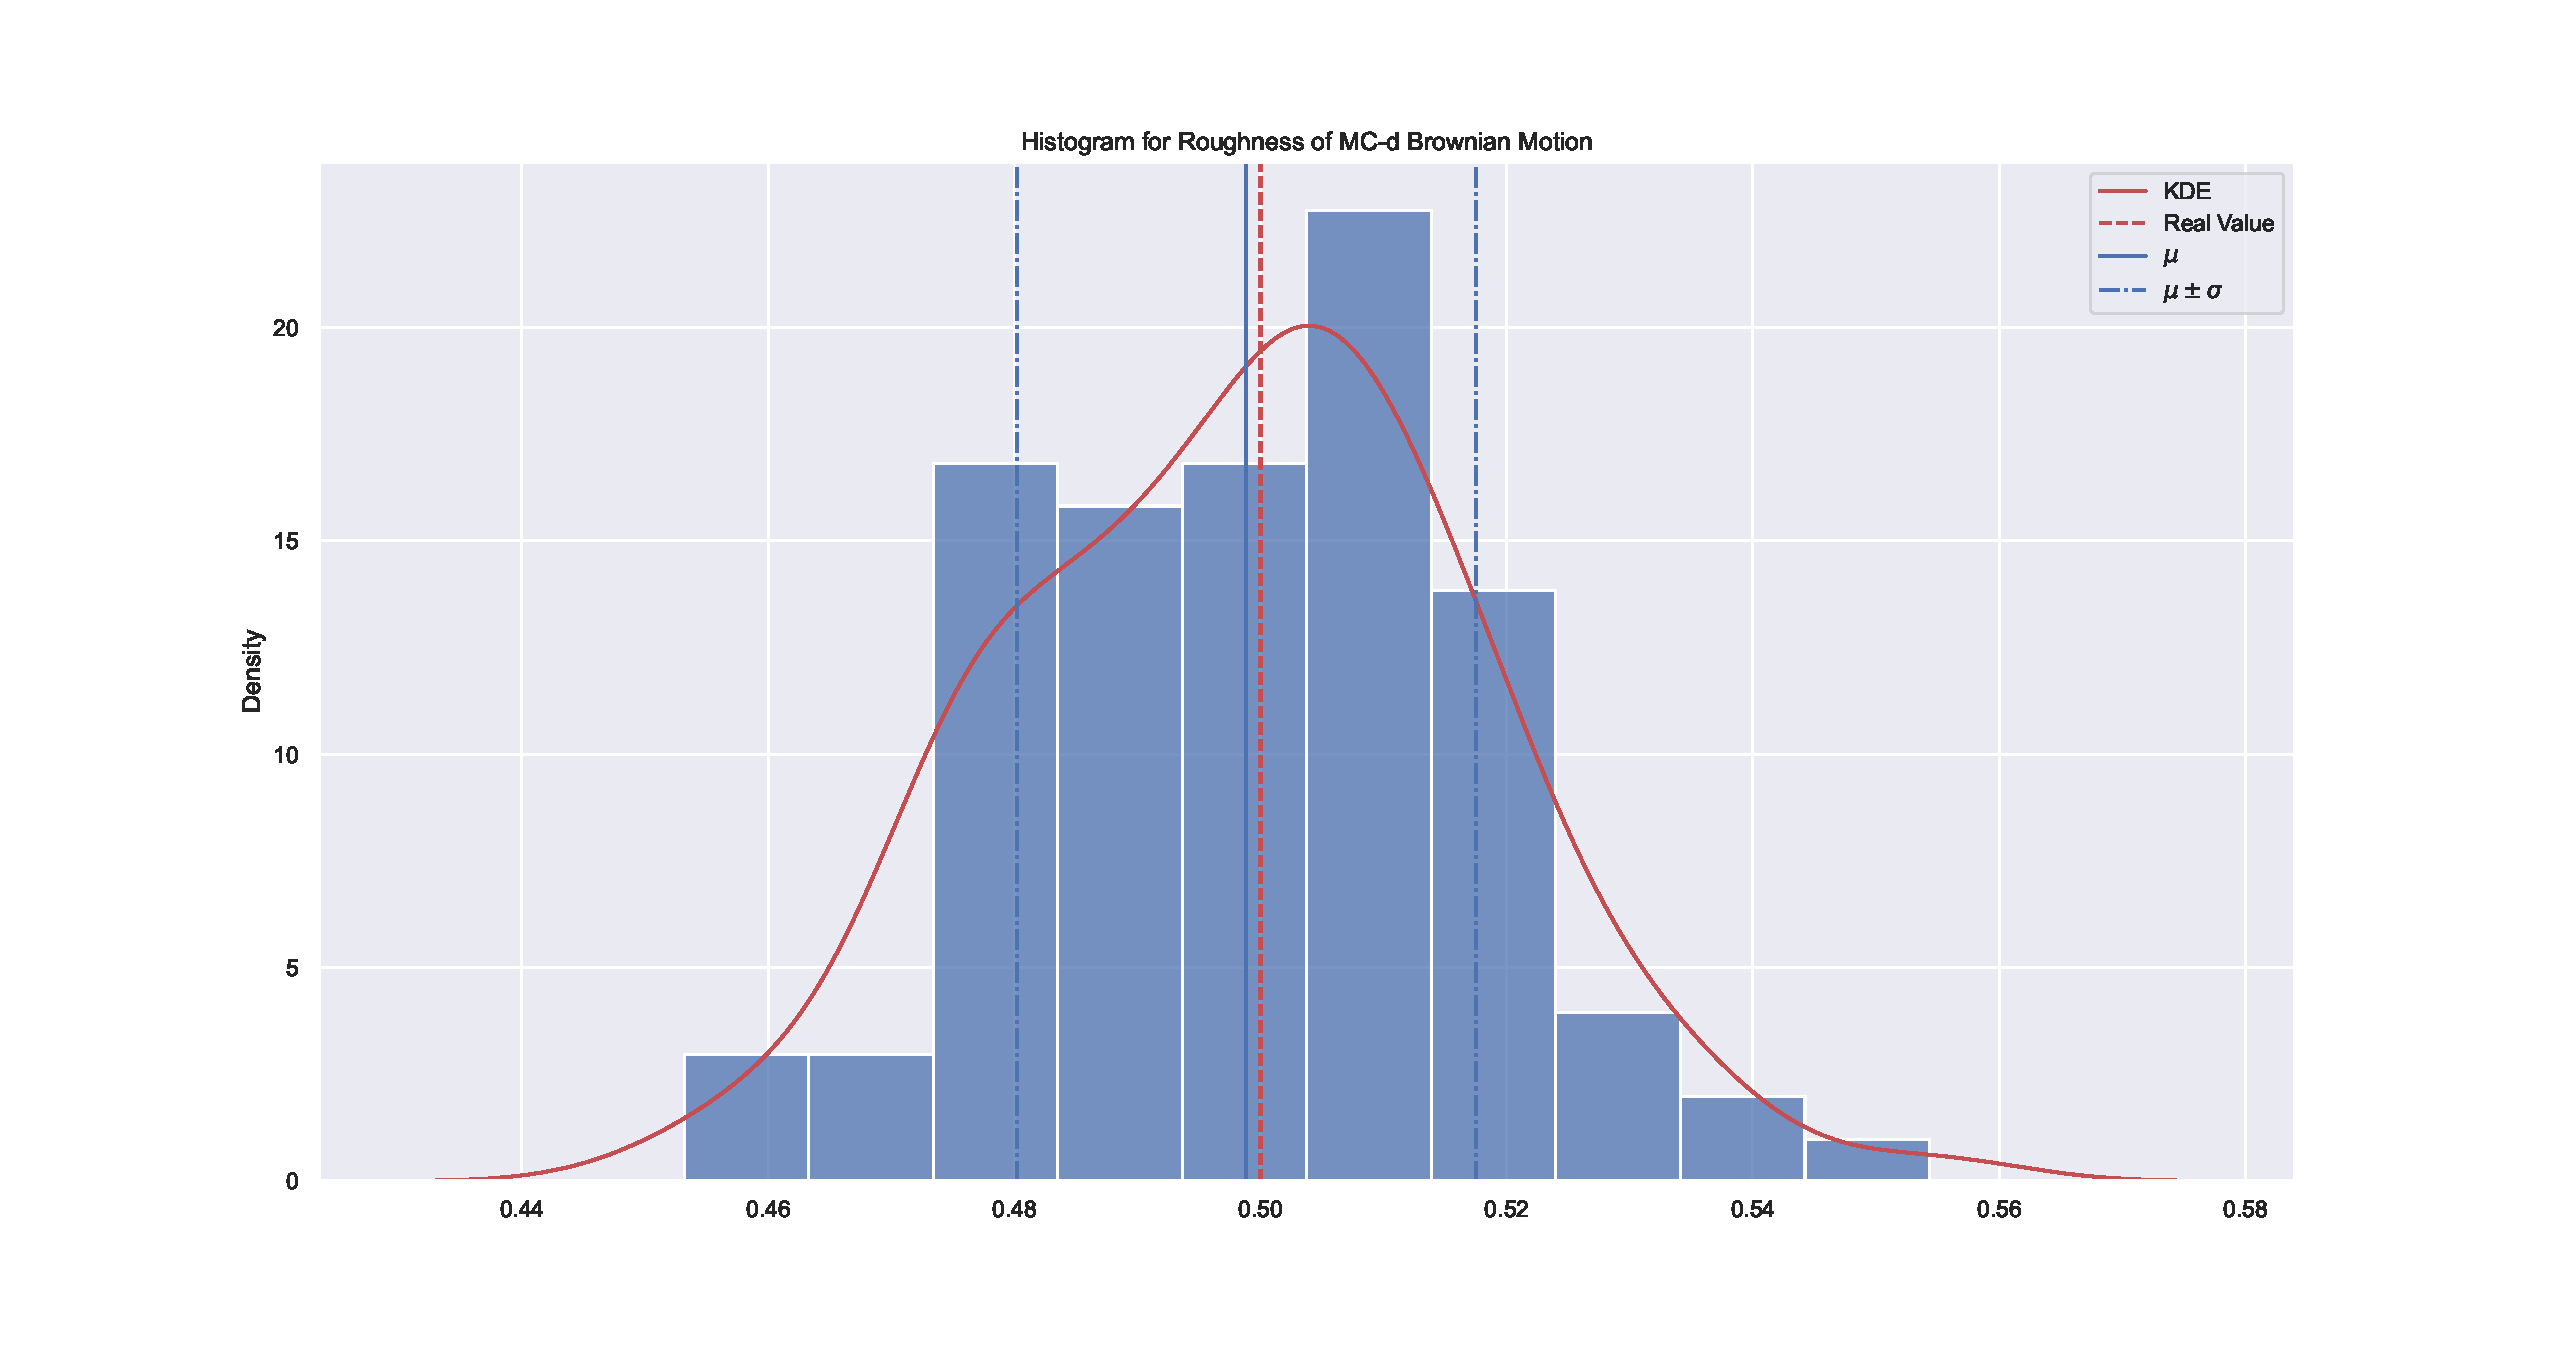
\includegraphics[width=\linewidth]{fig/Histogram for Roughness of MC-d Brownian Motion.pdf}
                \caption{Histogram for roughness of Brownian motion}
            \end{figure}

            We observe that the roughness index is equal to $0.4988$, which is a pretty good approximation.

        \subsubsection{Fractional Brownian motion (Davies-Harte method)}
            We considered four Hurst parameters for simulation: $0.15$, $0.35$, $0.55$, and $0.75$. We used the Davies-Harte method of generating 
            the fBm since this one is widely accepted as the most precise. We observe not the best approcsimations, but they are decent enough to be in $(\mu-\sigma, \mu+\sigma)$.
            \begin{figure}[htbp]
                \centering
                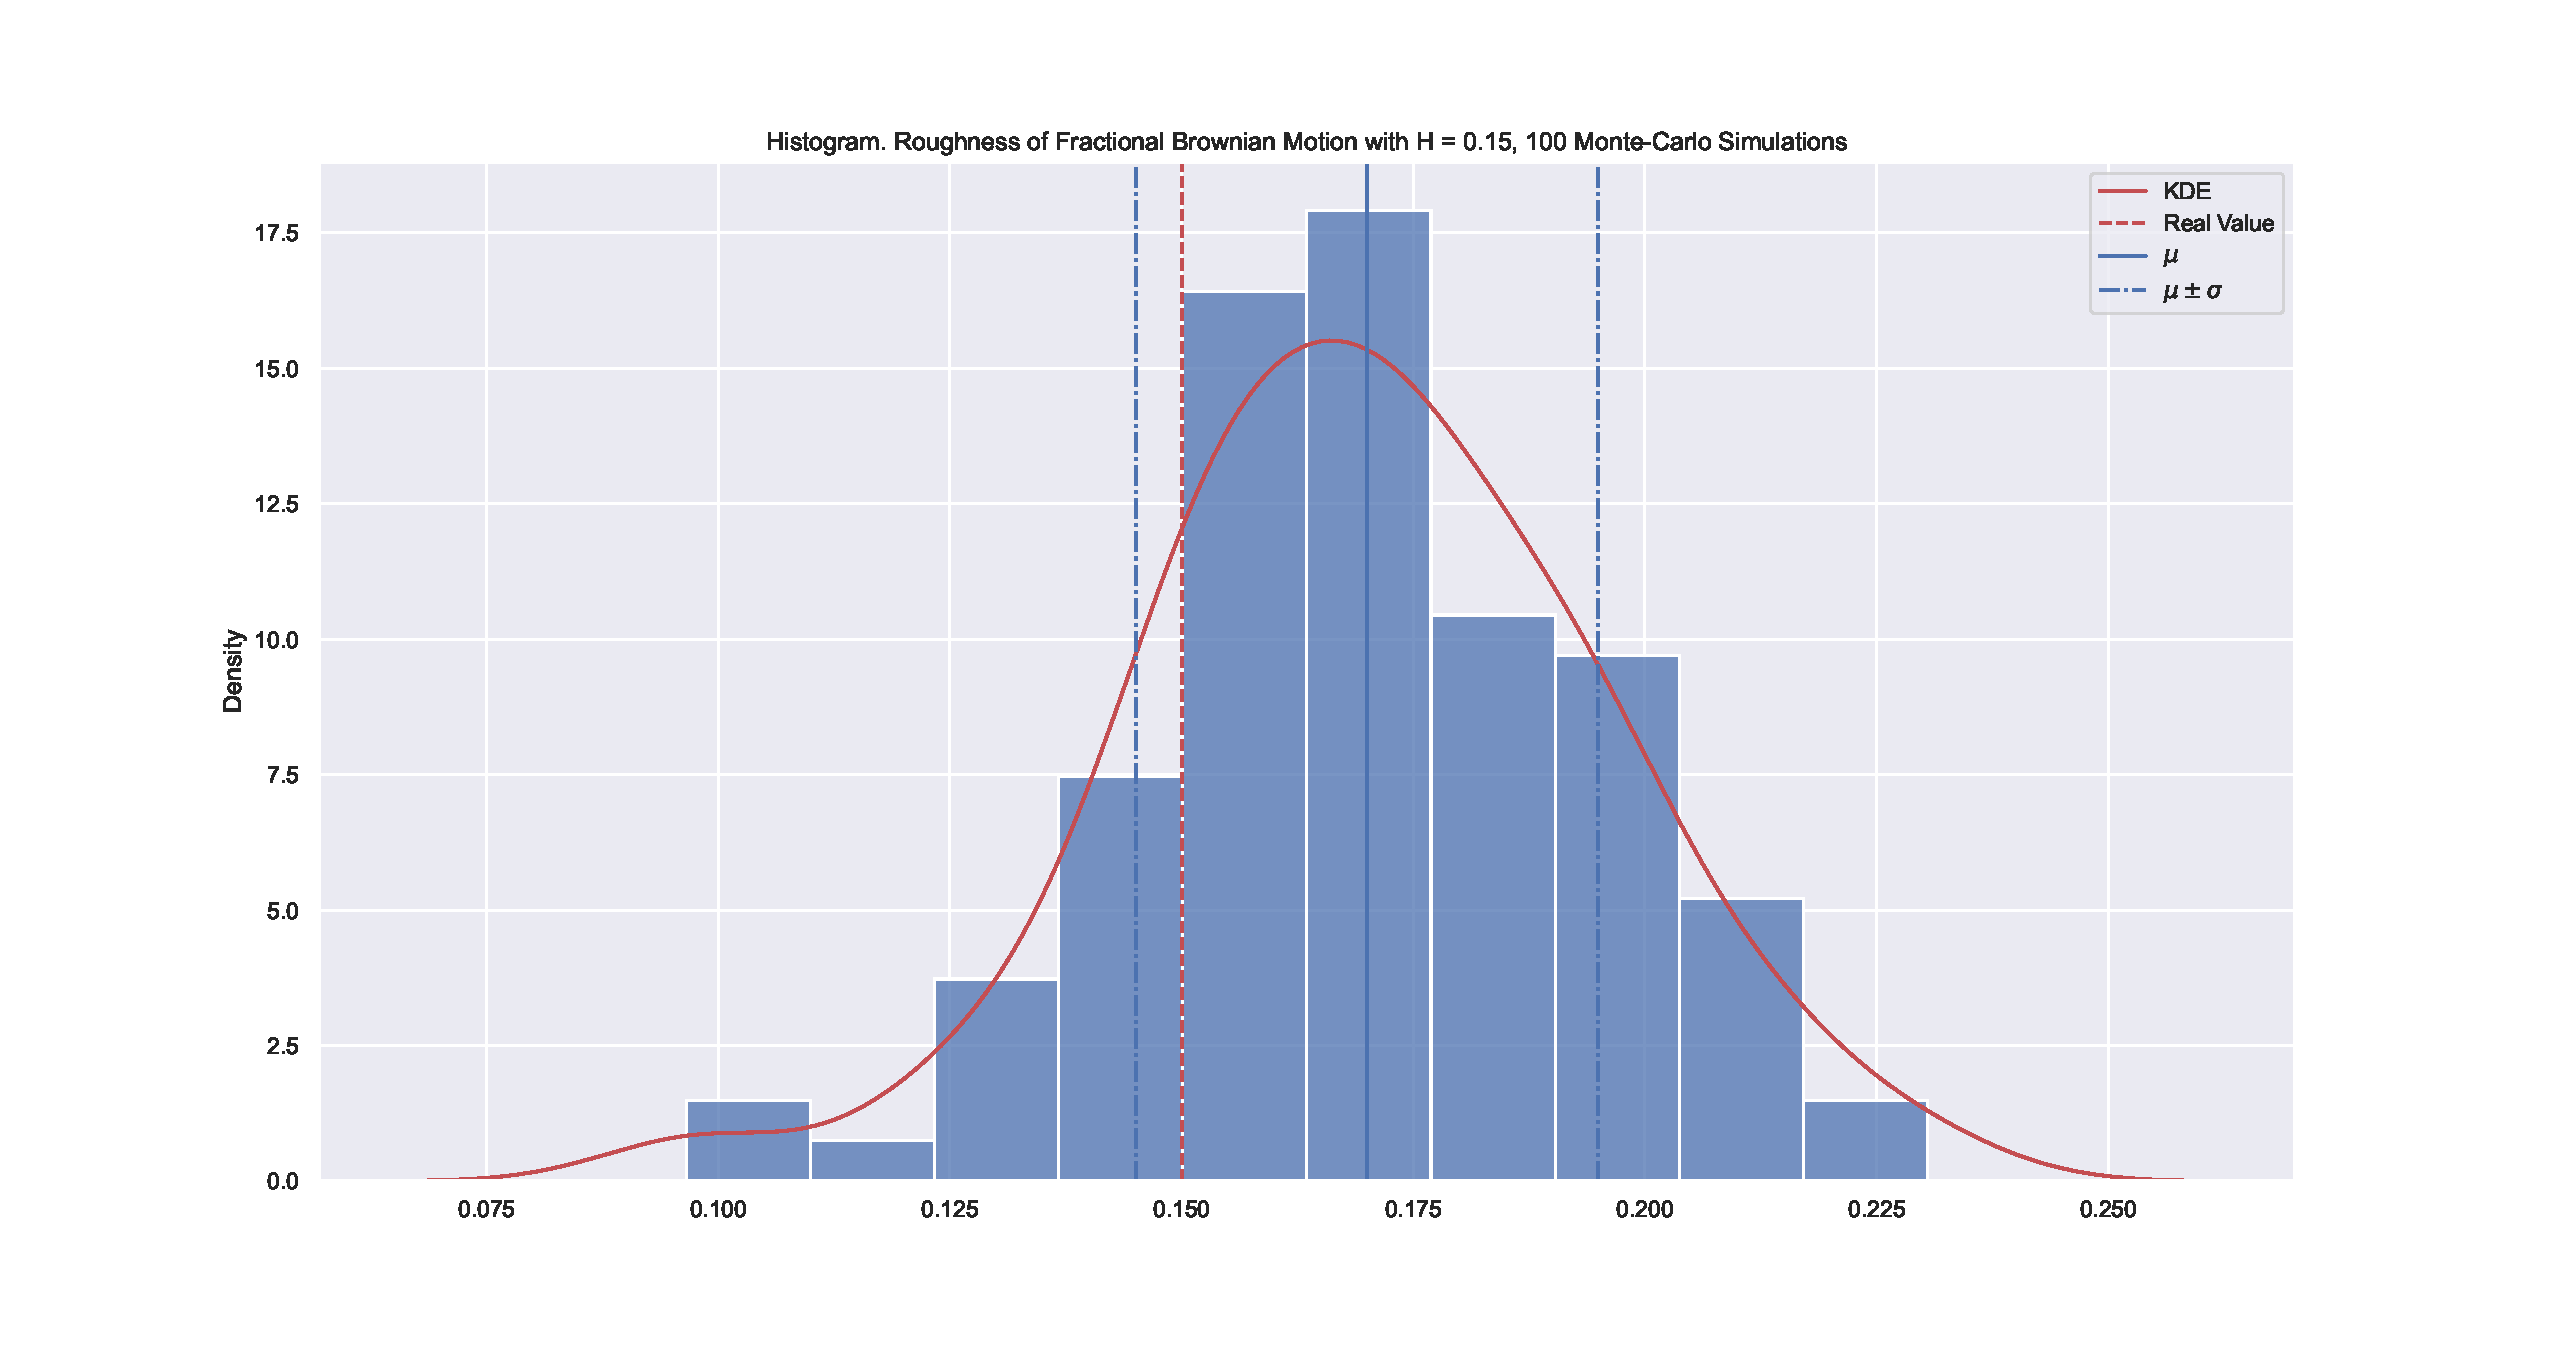
\includegraphics[width=\linewidth]{fig/Histogram. Roughness of Fractional Brownian Motion with H = 0.15, 100 Monte-Carlo Simulations.pdf}
                \caption{Histogram for roughness of fractional Brownian motion}
            \end{figure}
            \begin{figure}[htbp]
                \centering
                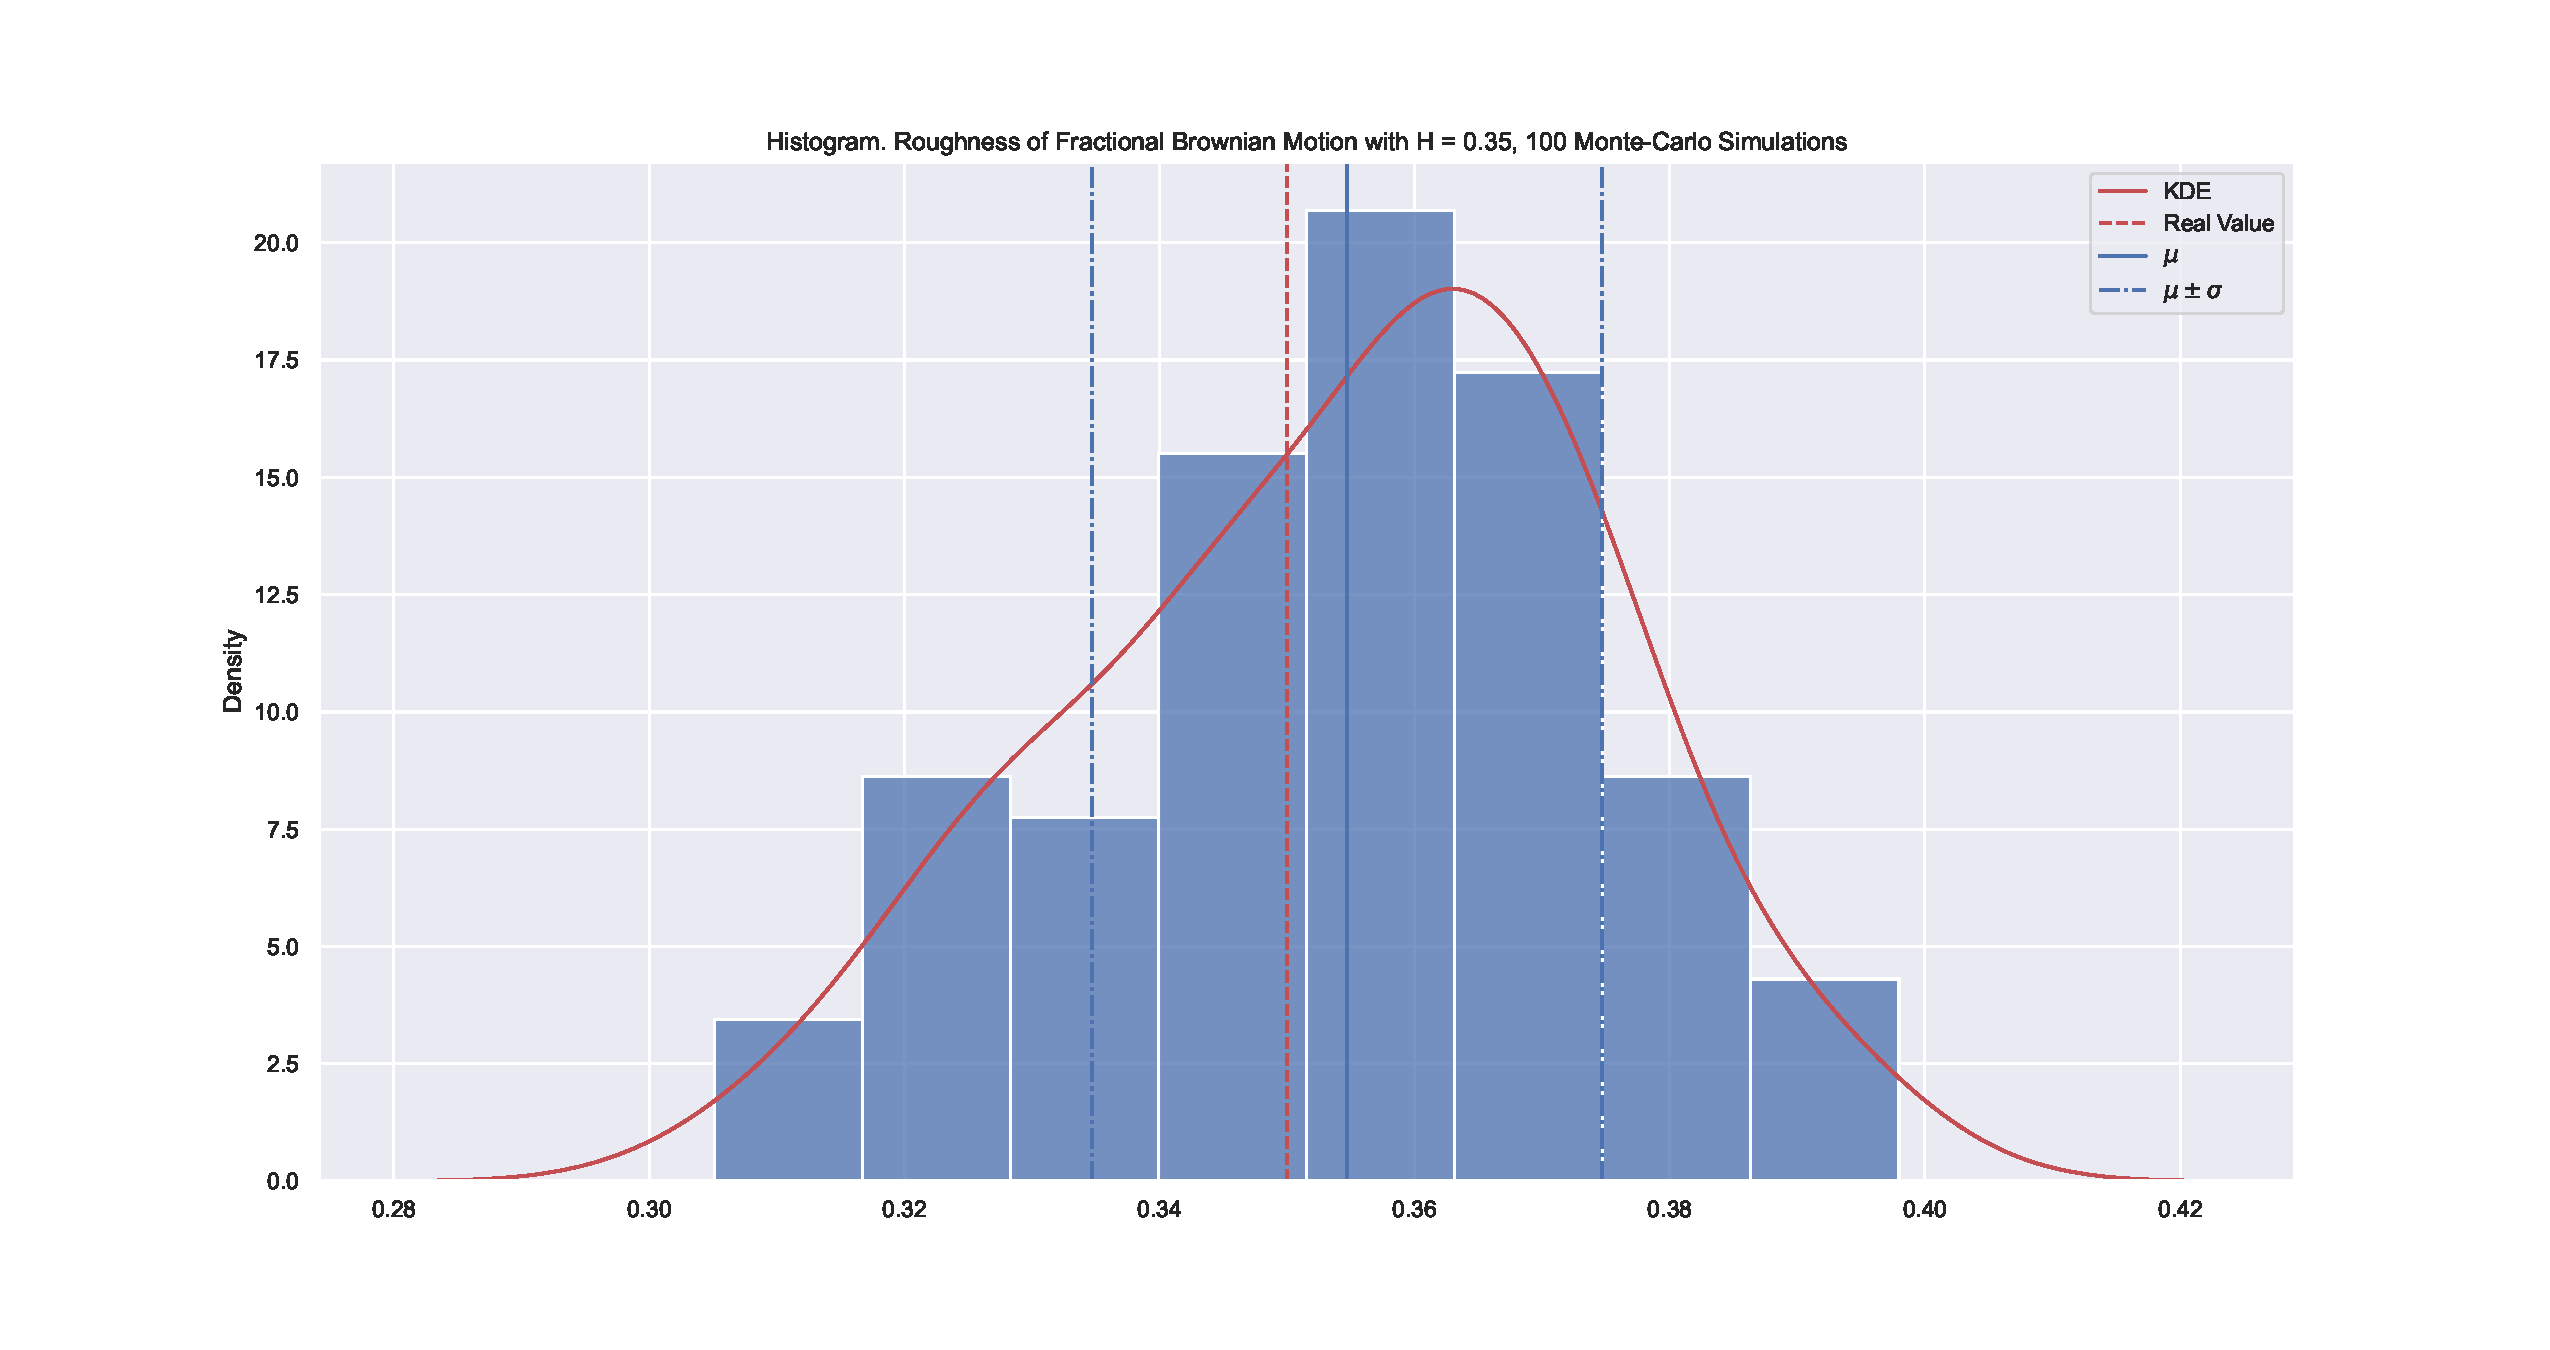
\includegraphics[width=\linewidth]{fig/Histogram. Roughness of Fractional Brownian Motion with H = 0.35, 100 Monte-Carlo Simulations.pdf}
                \caption{Histogram for roughness of fractional Brownian motion}
            \end{figure}
            \begin{figure}[htbp]
                \centering
                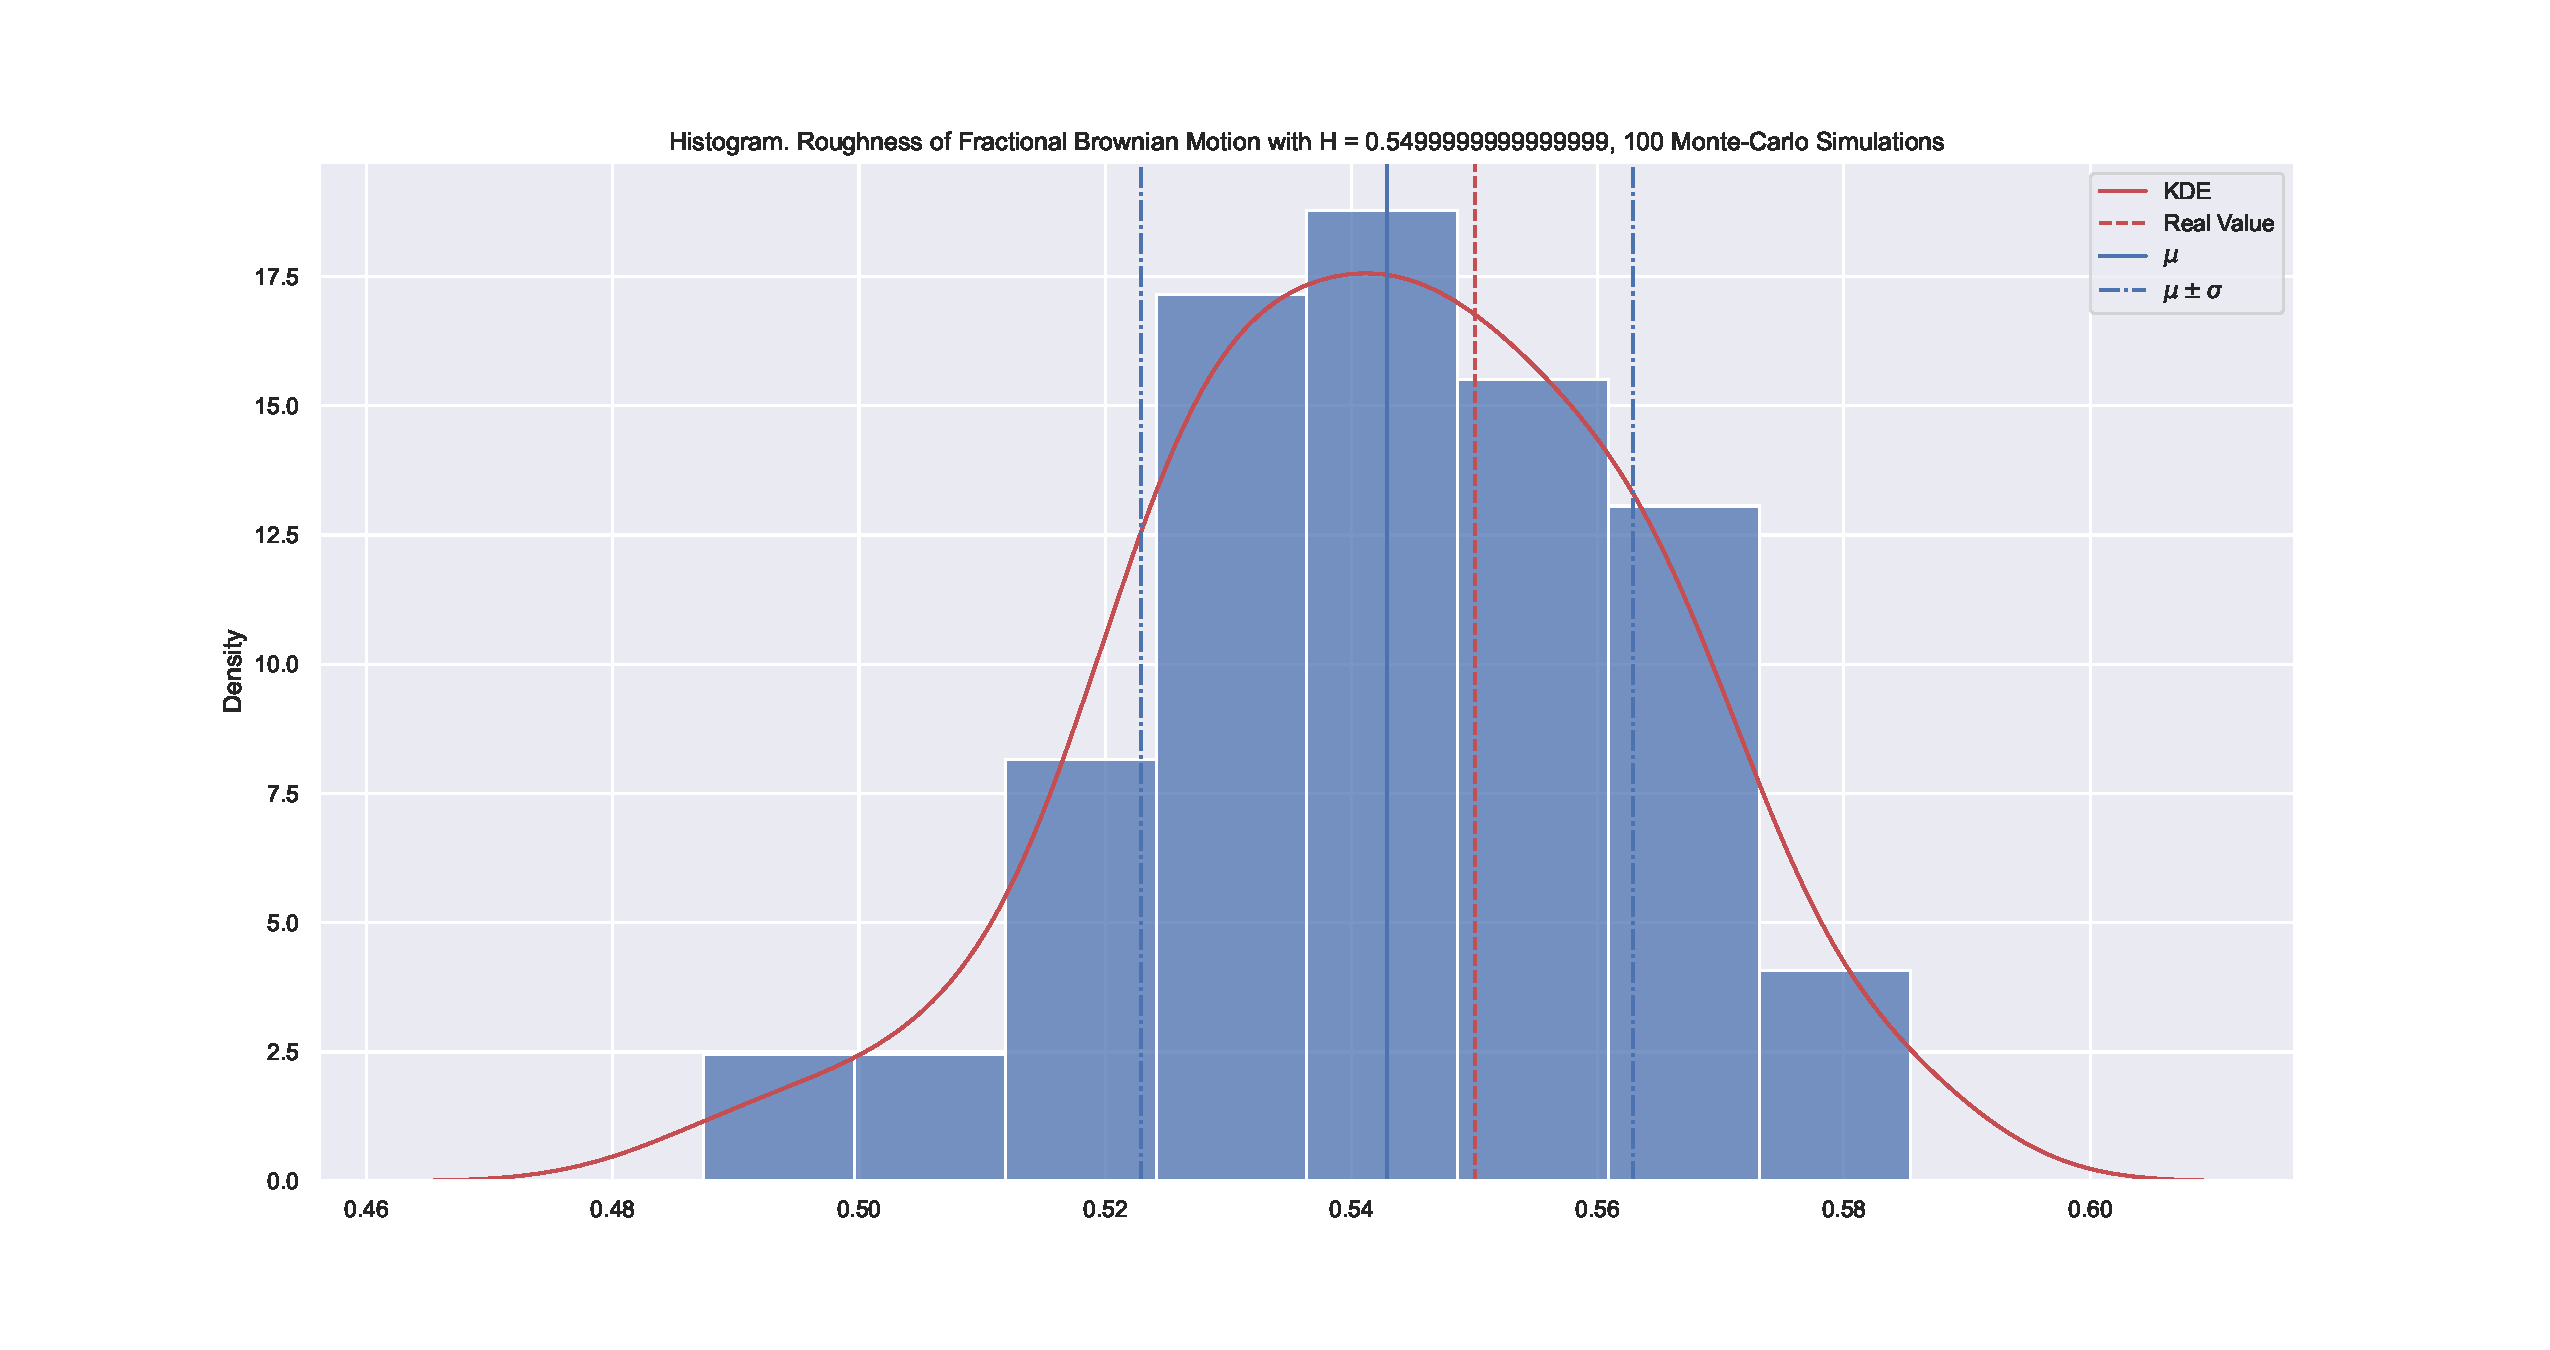
\includegraphics[width=\linewidth]{fig/Histogram. Roughness of Fractional Brownian Motion with H = 0.55, 100 Monte-Carlo Simulations.pdf}
                \caption{Histogram for roughness of fractional Brownian motion}
            \end{figure}
            \begin{figure}[htbp]
                \centering
                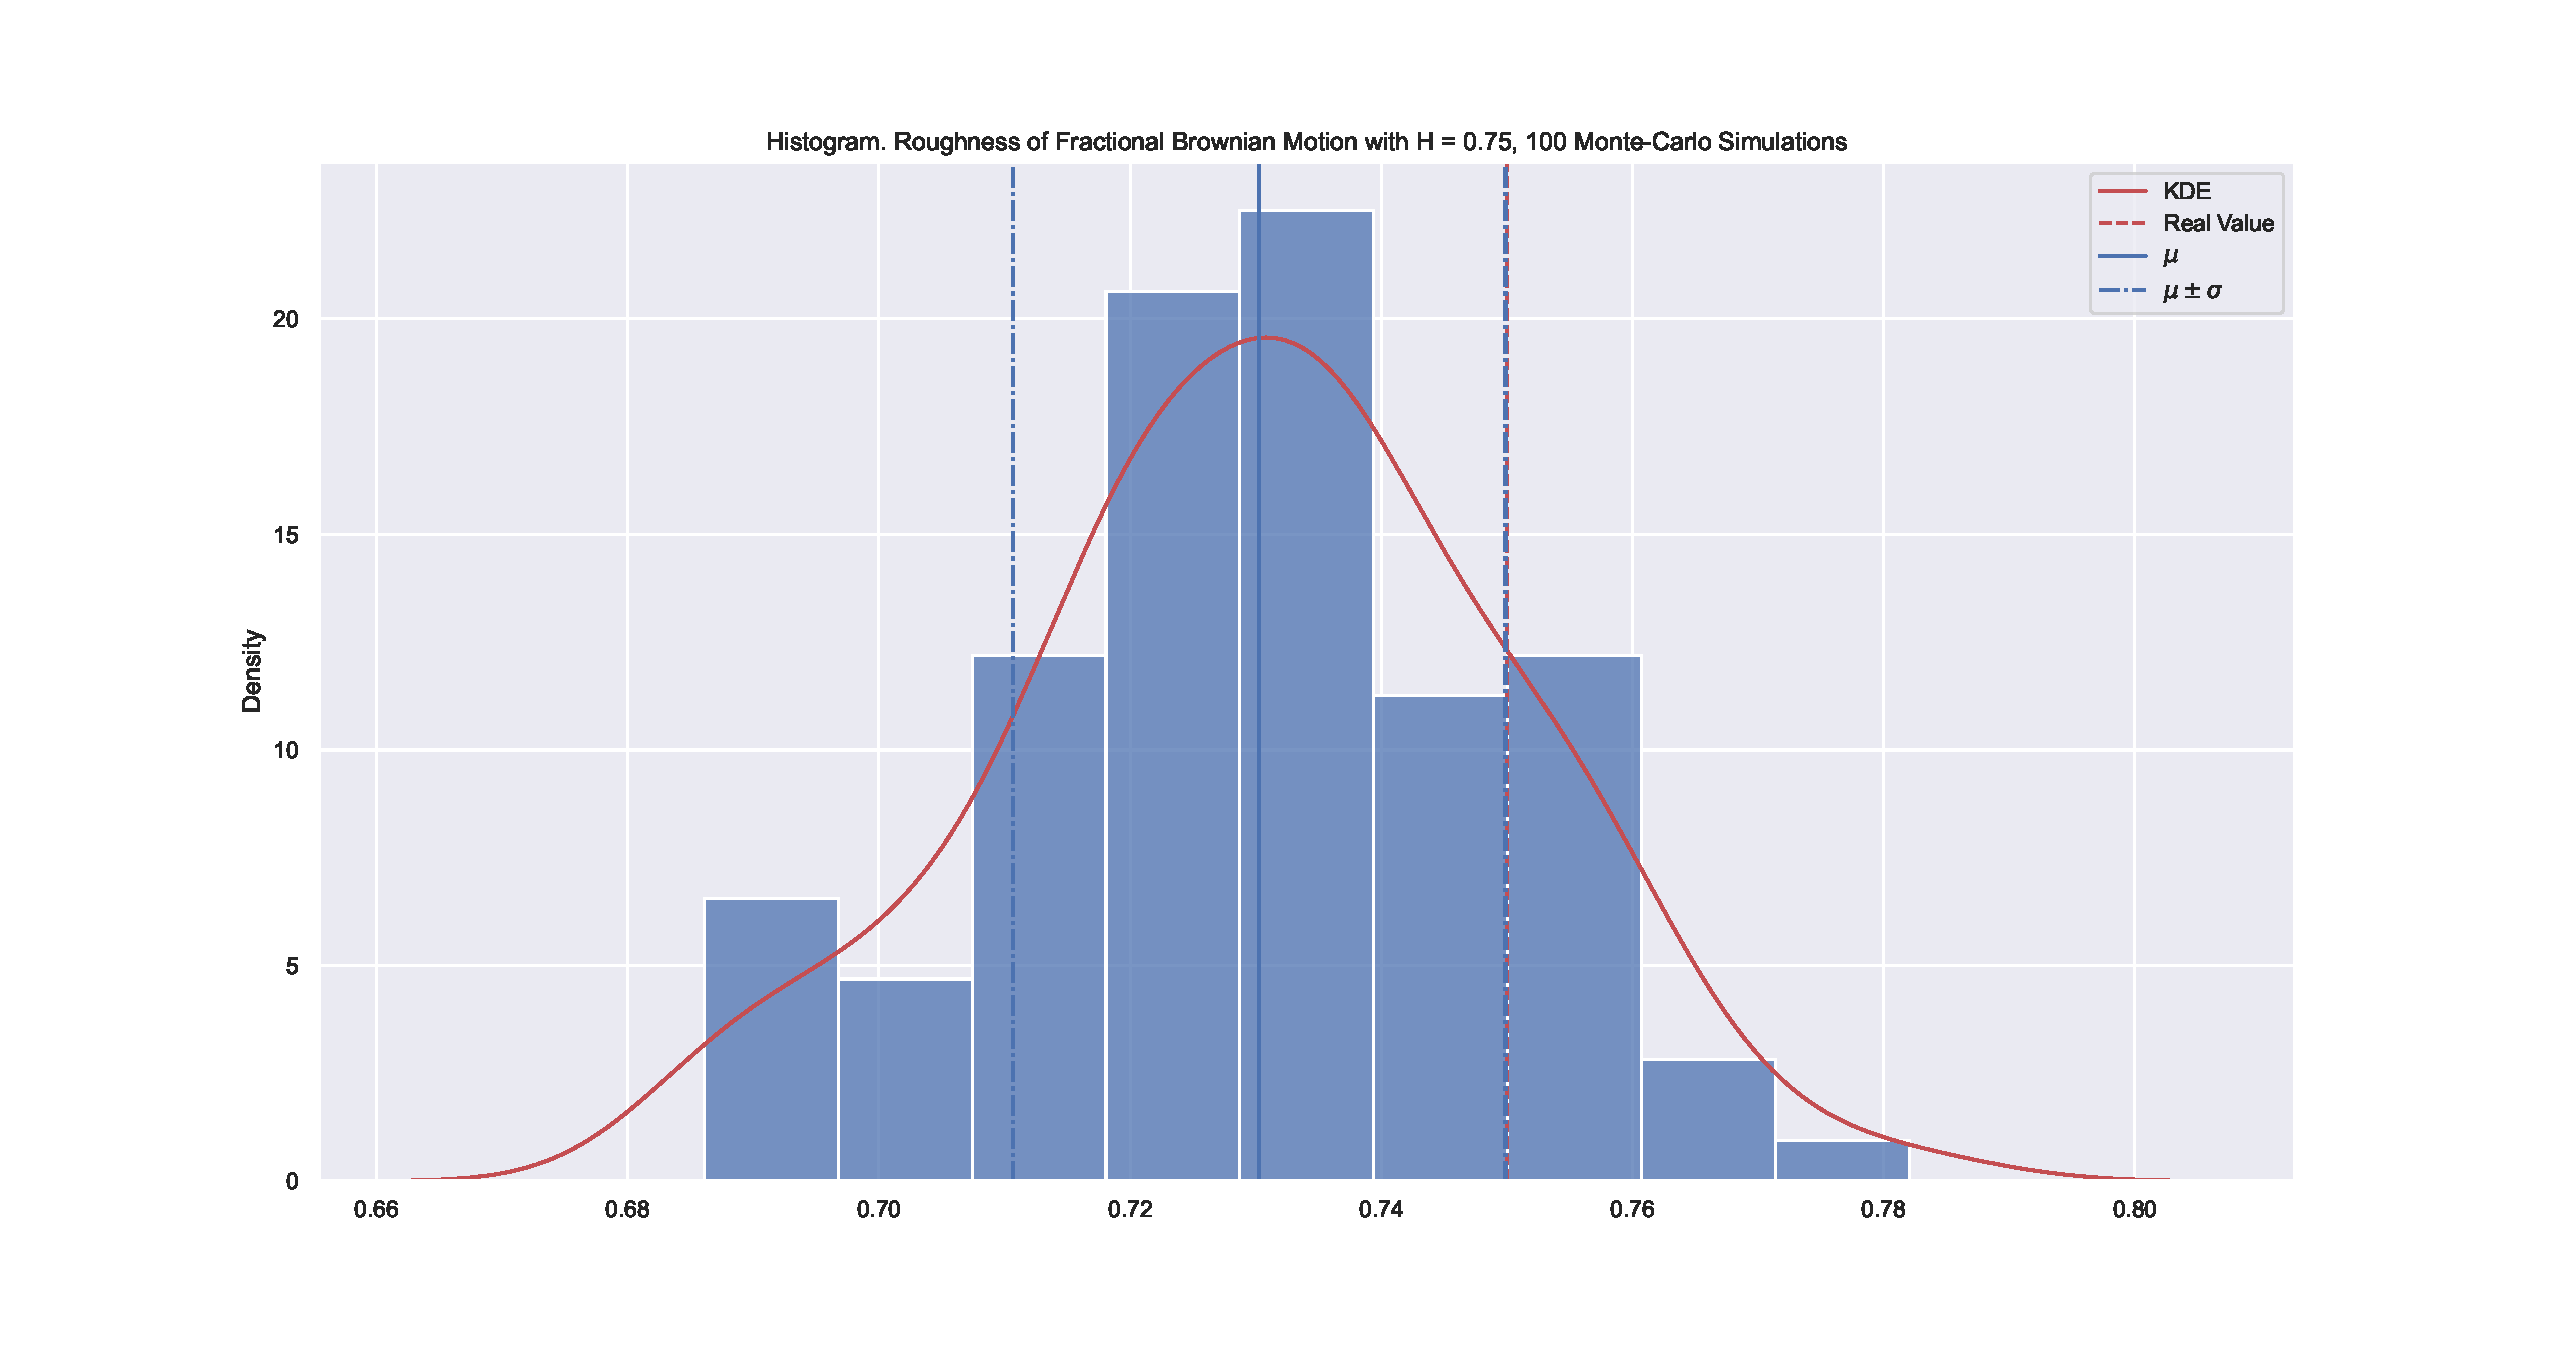
\includegraphics[width=\linewidth]{fig/Histogram. Roughness of Fractional Brownian Motion with H = 0.75, 100 Monte-Carlo Simulations.pdf}
                \caption{Histogram for roughness of fractional Brownian motion}
            \end{figure}

   \subsection{Heston stochastic volatility model}
        We observe that roughness estimations for instantaneous volatiltity and realized volatility significantly differ, which was described in the article for fOU processes.
    
    \begin{figure}[htbp]
        \centering
        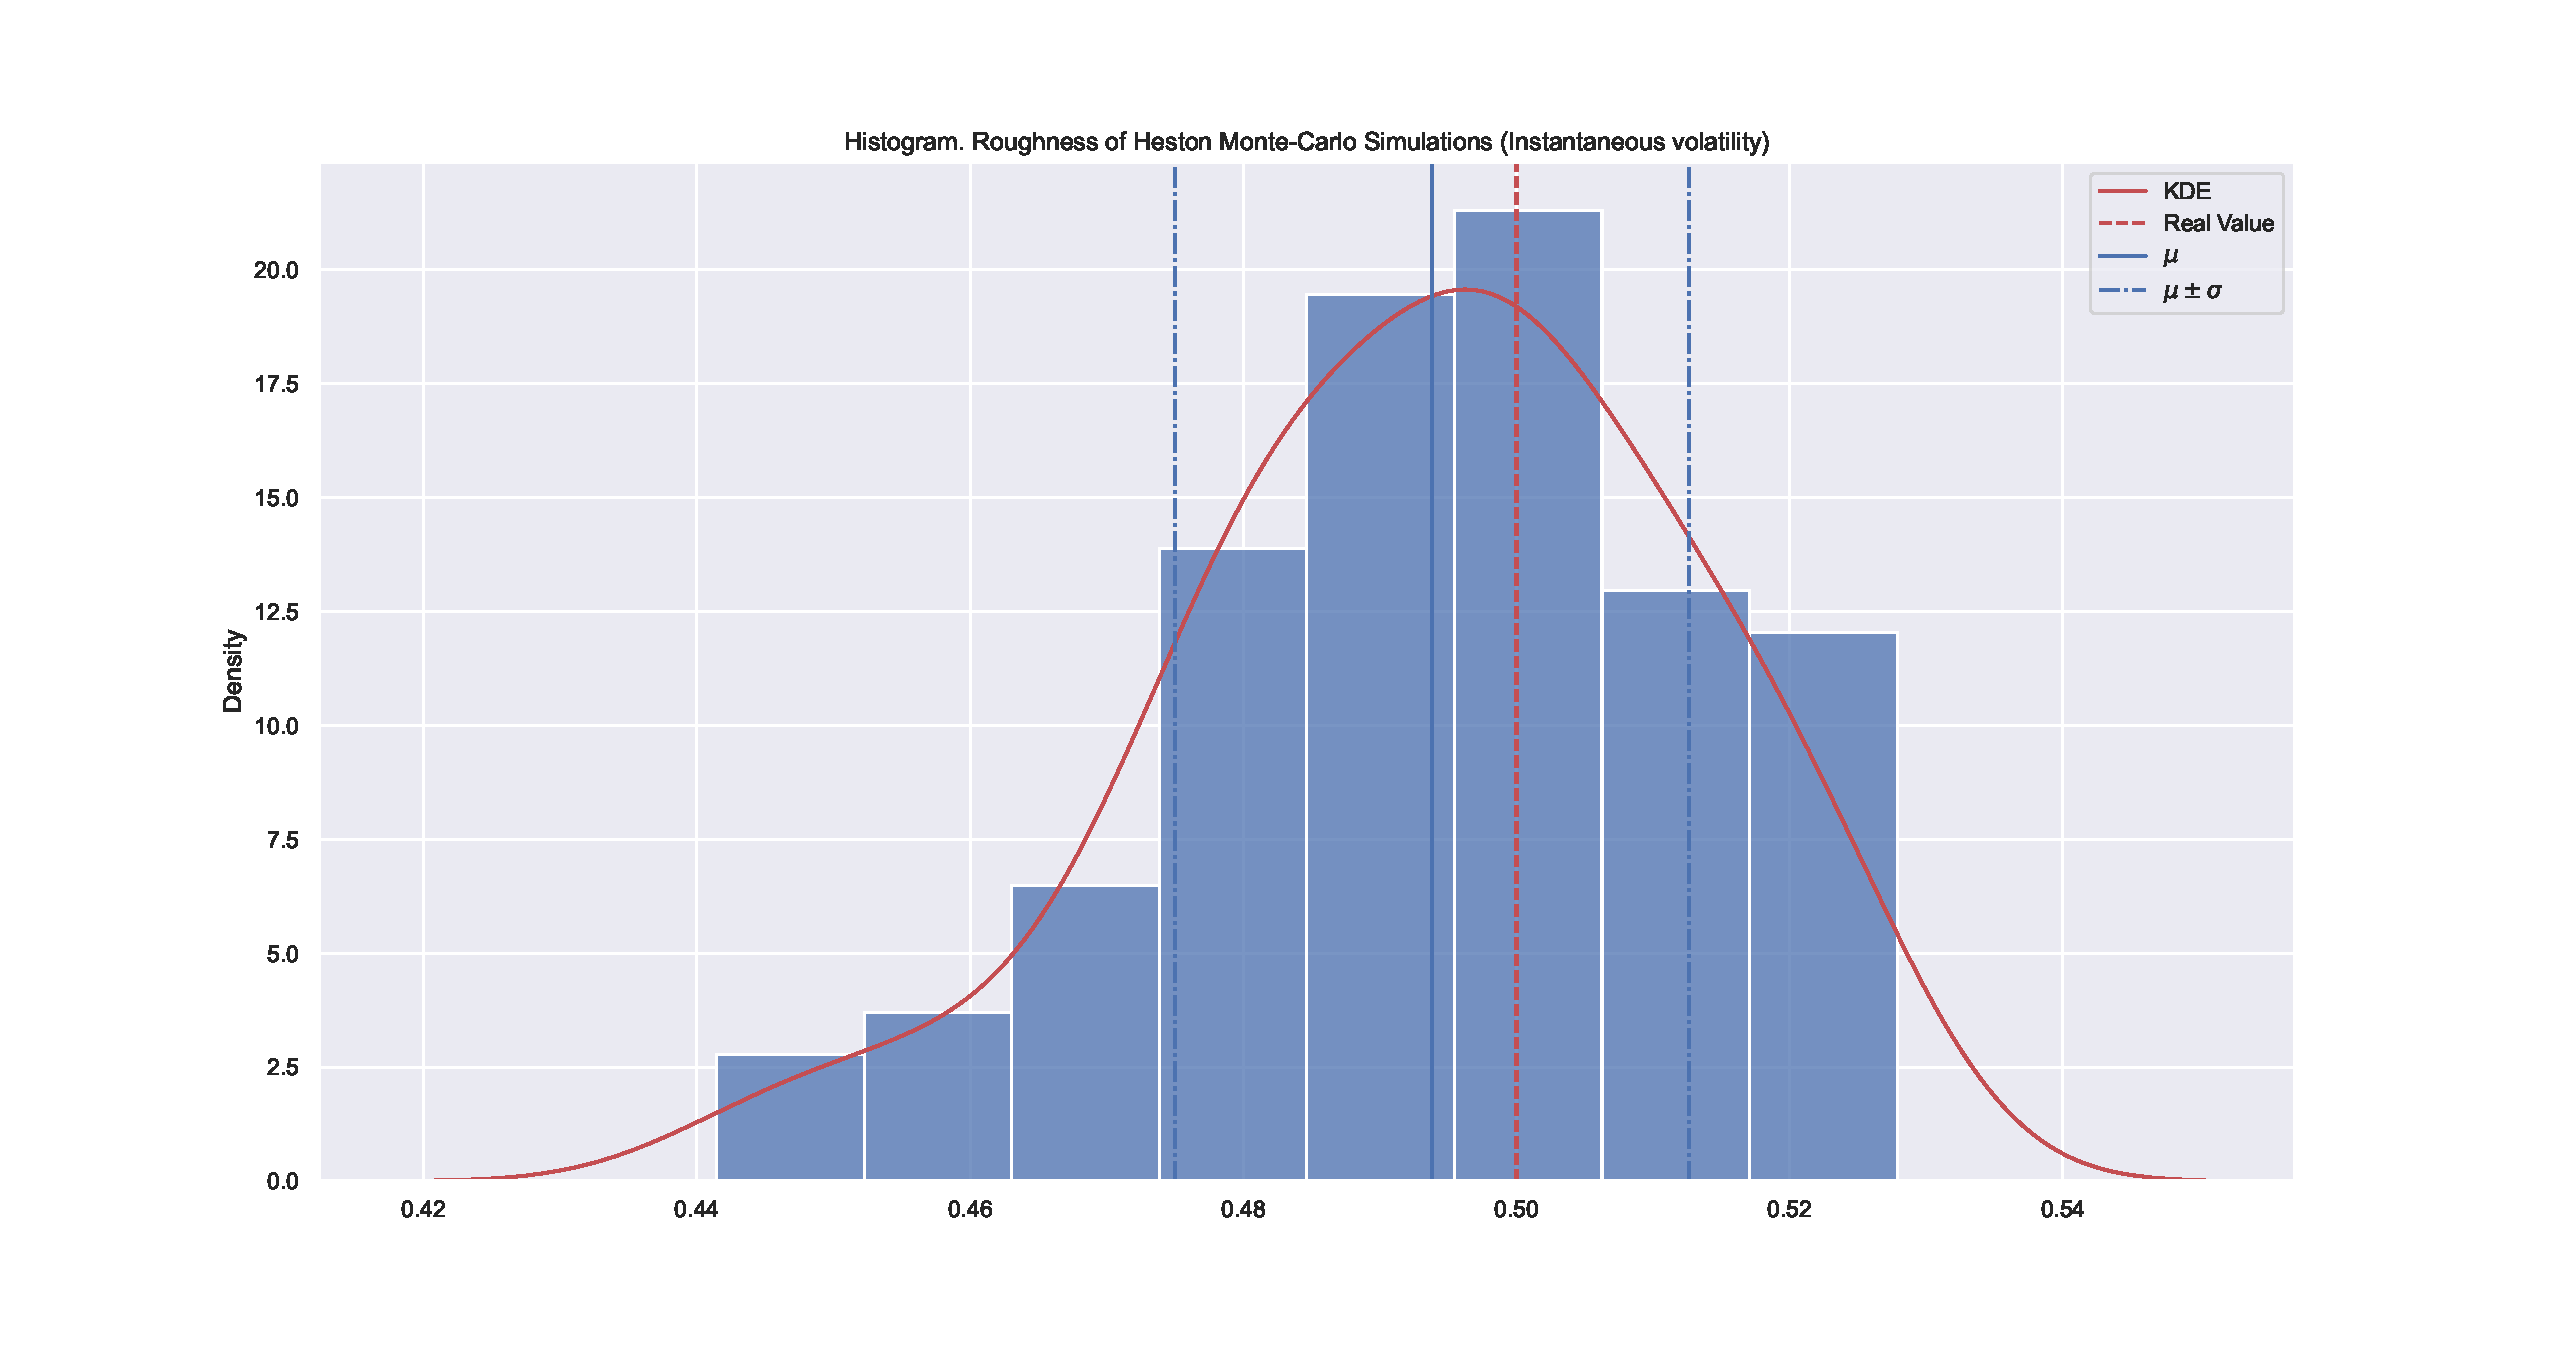
\includegraphics[width=\linewidth]{fig/Histogram. Roughness of Heston Monte-Carlo Simulations (Instantaneous volatility).pdf}
        \caption{Histogram for roughness of Heston SVM}
    \end{figure}
    \begin{figure}[htbp]
        \centering
        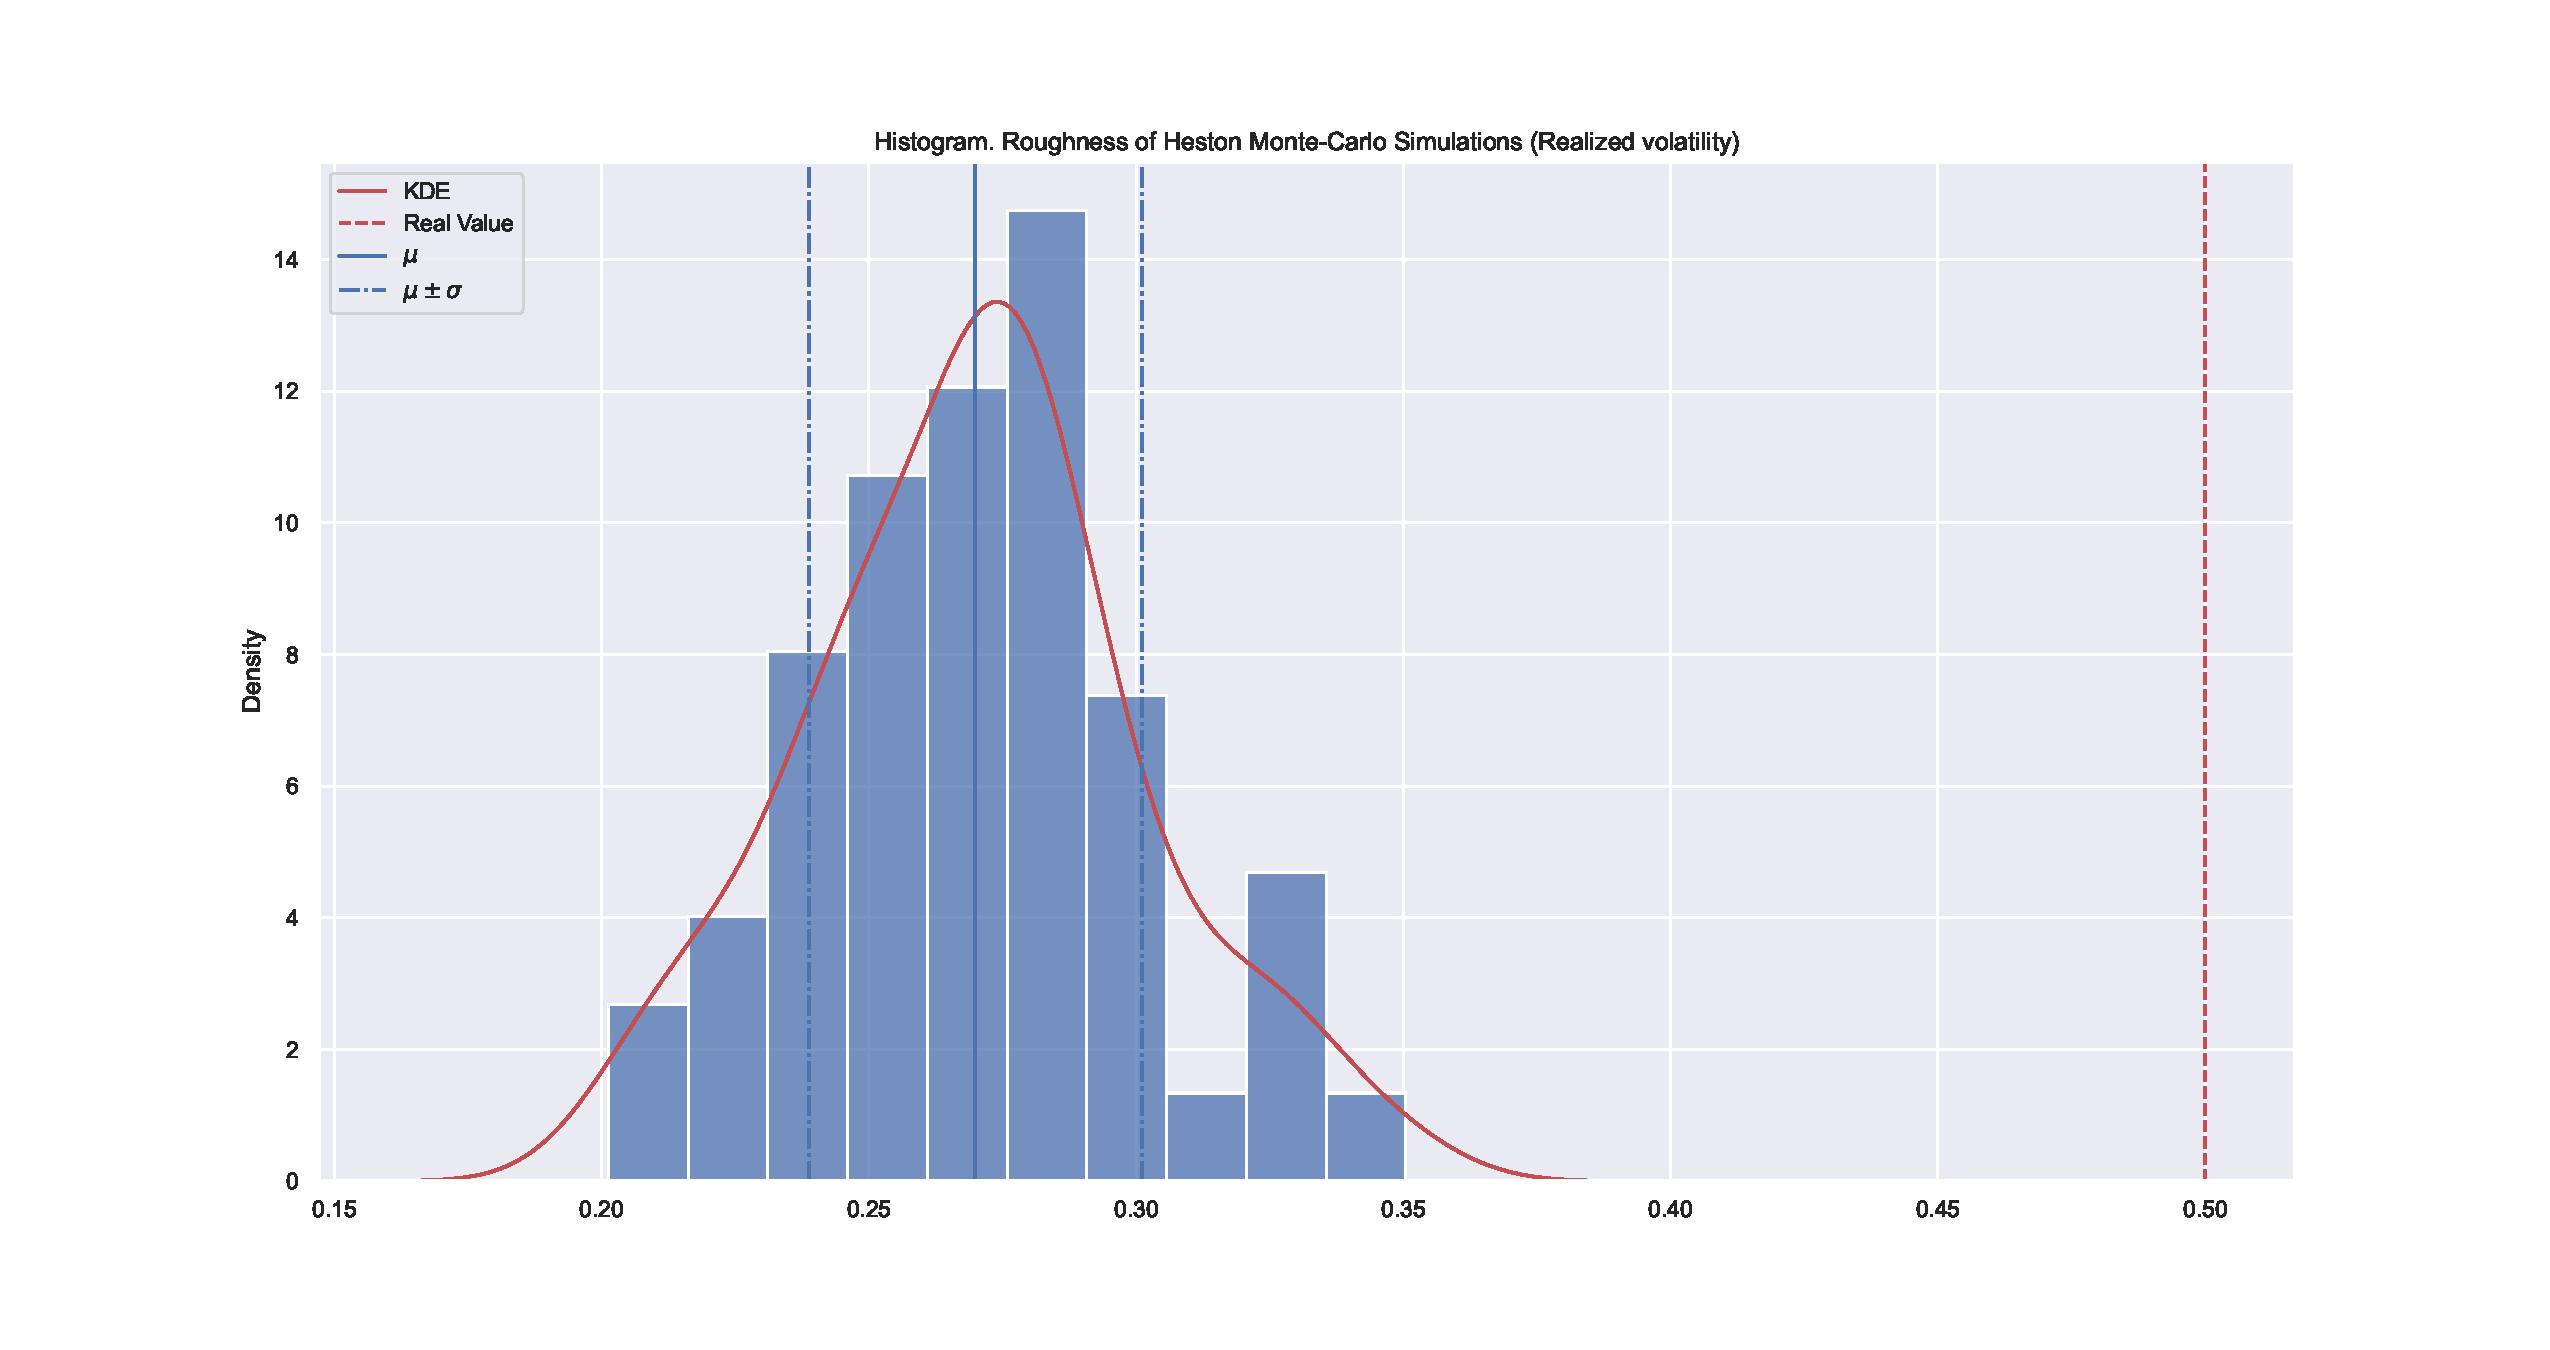
\includegraphics[width=\linewidth]{fig/Histogram. Roughness of Heston Monte-Carlo Simulations (Realized volatility).pdf}
        \caption{Histogram for roughness of Heston SVM}
    \end{figure}

\section{Roughness estimation of real-market data}

    Let us estimate the roughness of real-market data. 
    We are using the same Bloomberg data from Table \ref{table:hurst_est} (but without indexes).

    \begin{table}[h]
        \centering
        \begin{tabular}{|c|c|c|c|c|c|}
            \hline
            Ticker &  Roughness Index\\\hline
            \hline
            YNDX RX Equity & 0.372691\\\hline
            SBER RX Equity & 0.313109\\\hline
            VTBR RX Equity & 0.304677\\\hline
            MOEX RX Equity & 0.295378\\\hline
            LKOH RX Equity & 0.301795\\\hline
            GAZP RX Equity & 0.316125\\\hline
            FIVE RX Equity & 0.284704\\\hline
            \hline
            OGZD LI Equity & 2.968608\\\hline
            VTBR LI Equity & 0.306763\\\hline
            SBER LI Equity & 1.176616\\\hline
            LKOD LI Equity & 0.306061\\\hline
        \end{tabular}
        \caption{Roughness index estimation}
        \label{tab:roughness_index}
    \end{table}

    As we can see, modelless estimation of roughness differs from the Hurst parameter under RFSV (as Monte-Carlo simulations predicted).
